\chapter{Автоматическое дифференцирование}

Лектор: Алексей Сергеевич Забашта

\section{Сведение задачи обучения к задаче дифференцирования}

Задача машинного обучения состоит из трех частей:
\begin{itemize}
    \item Набор данных (выборка)
    \item Модель
    \item Функция ошибки
\end{itemize}

Введем необходимую терминологию:
\begin{enumerate}
    \item Обучаемая функция: $f(x_1, x_2, ..., x_n, a_1, a_2, ..., a_m): \R ^{n + m}\to\R ^k$, где $n$ --- число признаков, $m$ --- число обучаемых параметров, $k$ --- число предсказываемых (целевых) признаков.
    \item Набор данных: $D=\{(\vec{x}_i, \vec{y}_i)\}$.
    \item Функция ошибки: $E(\widehat{y}_1, ..., \widehat{y}_{|D|}, y_1, ..., y_{|D|})$, где $\widehat{y}_i$ --- предсказанный вектор для $i$-го объекта, а $y_i$ --- реальный. Например, $$\mathrm{MSE}(\widehat{y}_1, ..., \widehat{y}_{|D|}, y_1, ..., y_{|D|})=\frac{1}{|D|\cdot k}\sum_{i=1}^{|D|}\sum_{j=1}^k(y_{i,j} - \widehat{y}_{i,j})^2$$.
    \item Режим обучения: $E_{train}(a_1,...,a_m)=E(f(\vec{x}_1, \vec{a}),...,f(\vec{x}_{|D|}, \vec{a}),y_1,...,y_{|D|})$. Переменные $x$ зафиксированы функцией ошибки, а переменные $a$ изменяются в процессе \textit{минимизации}.
    \item Режим предсказания: $f_{predict}(x_1,...,x_n)=f(x_1,...,x_n,a_1,...a_m)$. Переменные $x$ изменяются от запроса к запросу, а переменные $a$ зафиксированы в процессе обучения.
\end{enumerate}

Задачу машинного обучения можно свести к задаче оптимизации. Решать её далее можно градиентным спуском или эволюционным алгоритмом (однако, когда известен градиент, лучше использовать градиентный спуск).

\begin{remark}
    Вычислять градиент можно автоматически.
\end{remark}

\begin{remark}
    Если функция не выпуклая, то можно:
    \begin{itemize}
        \item Предположить, что функция ошибки почти выпуклая;
        \item Обновлять параметры в градиентном спуске более хитрыми методами;
        \item Попробовать на практике.
    \end{itemize}
\end{remark}

\section{Дифференцирование составных функций по графу вычислений}

\begin{definition}
    \textbf{Составная функция} --- функция, которая состоит из элементарных функций, для которых мы умеем вычислять производную. Как правило, описывается графом вычислений.
\end{definition}

\begin{definition}
    \textbf{Сложная функция} --- функция, тип значения которой отличен от скаляра, может быть вектором, матрицей и так далее.
\end{definition}

Если собрать из нескольких функций одну, то её размер может экспоненциально расти --- это наивное вычисление функции. Наш путь --- это граф вычислений.

\begin{definition}
    \textbf{Статический граф} вычислений строится до вычисления функции. Можно заранее выполнить какие-то оптимизации.
\end{definition}

\begin{definition}
    \textbf{Динамический граф} вычислений строится во время вычисления функции и является более гибким.
\end{definition}

Если выполнять вычисление производной по графу вычислений от параметров к последней вершине, нам сначала потребуется для всех вершин в графе посчитать производную всех вершин по $x_1$, затем по $x_2$ и так далее. Это \textbf{forward-подход}. Однако можно считать производную $f$ по всем вершинам графа, начиная с того, что $\dv{f}{f}=1$, и пересчитывая от конца к вершинам-параметрам. Тогда потребуется всего один проход по графу - это \textbf{backward-подход}.

\begin{remark}
    На практике под термином \textbf{forward} понимают вычисление функции (так как forward-подход к вычислению производной бесполезен), а под \textbf{backward} - вычисление производной.
\end{remark}

Элементарный дифференцируемый блок (см. рисунок 2.6) может запоминать $X$ и $Y$, а также любые другие промежуточные значения, необходимые при пересчёта производной. Блоку для пересчёта производной целевой функции не нужно знать всю функцию целиком.

\begin{figure}[h]
    \centering
    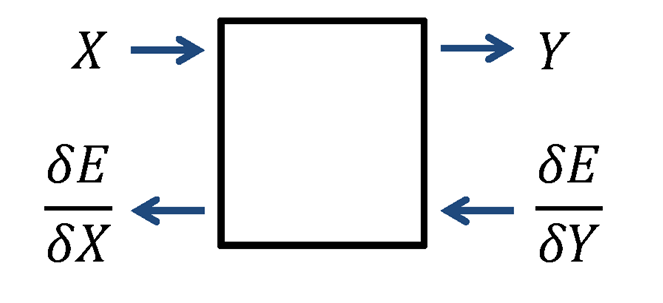
\includegraphics[scale=0.3]{./images/elementary-differential-block.png}
\end{figure}

\begin{remark}
    Тип и размер $X$ совпадает с $\pdv{E}{X}$, а $Y$ с $\pdv{E}{Y}$.
\end{remark}

Можно составлять композиции блоков, чтобы получать новые блоки:
\begin{figure}[h]
    \centering
    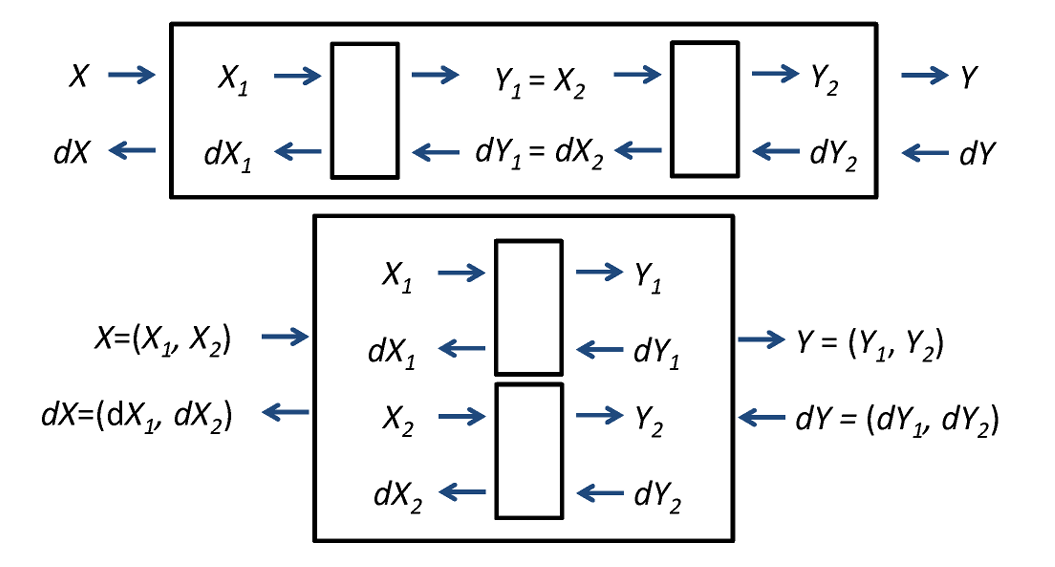
\includegraphics[scale=0.5]{./images/blocks-composition.png}
\end{figure}

Пересчет производной производится по цепному правилу и его обобщению:
\[
    (f(g(x)))'=g'(x)\cdot f'(g(x)) \Longrightarrow \pdv{f}{x} = \pdv{g}{x} \pdv{f}{g}
\]
\[
    \pdv{f(g_1(x), g_2(x),...,g_n(x))}{x} = \sum_i \pdv{f}{g_i}\pdv{g_i}{x}
\]

Таким образом, можно сформулировать алгоритм дифференцирования по графу вычислений:
\begin{enumerate}
    \item Вычисляем составную функцию $Q$, сохраняя граф вычислений $G=(V, E) : (u, v) \in E$, если вершина (блок) $v$ напрямую зависит от $u$;
    \item Для всех вершин $v$ устанавливаем:
    \[
        \pdv{Q}{v}=I[v=Q]
    \]
    \item Для каждого ребра $(u, v)\in E$ в обратном порядке вычисления целевой функции:
    \begin{itemize}
        \item Если $v$ --- это простая функция, то
        \[
            \pdv{Q}{u} \pluseq \pdv{Q}{v} \cdot \pdv{u}{v}
        \]
        \item Если $v$ --- это сложная функция (вычисляется абстрактным блоком):
        \[
            \pdv{Q}{u} \pluseq df_{u\to v}\left(\pdv{Q}{v}\right)
        \]
    \end{itemize}
\end{enumerate}

\begin{remark}
    Важно, что в данных правилах используется оператор $\pluseq$, а не $=$. Это связано с тем, что $(u, v)$ может быть не единственным ребром из вершины $u$, а по обобщению правила цепочки по всем таким ребрам производные необходимо суммировать.
\end{remark}

\begin{remark}
    В данном контексте $df_{u\to v}$ означает пересчет производной из $\pdv{Q}{v}$ в $\pdv{Q}{u}$.
\end{remark}

\begin{example}
    Дифференцирование простых функций:
    \begin{itemize}
        \item Сумма:
        \[
            y = \sum x_i \Longrightarrow dx_i \pluseq dy
        \]
        \item Произведение:
        \[
            y = \prod x_i \Longrightarrow dx_i \pluseq  dy \cdot \prod_{j\ne i} x_j
        \]
        \item Применение функции:
        \[
            y = f(x) \Longrightarrow dx \pluseq dy \cdot f'(x).
        \]
    \end{itemize}
\end{example}

\begin{figure}[h]
    \centering
    \includesvg[scale=0.27]{\detokenize{./images/example-differentiation.svg}}
    \caption{Пример дифференцирования функции $F=\frac{\sin(x+y)}{x\cdot y}$}
\end{figure}

\begin{remark}
    В данном контексте запись $dx$ --- это сокращение для $\pdv{Q}{x}$, где $Q$ --- это конечная вершина в графе. Таким образом, последнее правило можно переписать так:
    \[
        y = f(x) \Longrightarrow \pdv{Q}{x} \pluseq \pdv{Q}{y} \cdot \pdv{y}{x} = \pdv{Q}{y} \cdot f'(x). 
    \]
\end{remark}

\section{Дифференцирование сложных функций}

До этого речь шла о скалярных функциях. Для сложных функций всё сложнее и общего алгоритма нет. Есть отдельный матричный подход. Однако, можно рассматривать частные случаи.

\begin{example}
    Если сложное скалярное произведение можно посчитать следующей функцией:
    \begin{lstlisting}
        for i ...
            for j ...
                for k ...
                    if (...)
                        x = f(i, j, k)
                        y = g(i, j, k)
                        z = h(i, j, k)
                        c[z] += a[x] * b[y]
    \end{lstlisting}
    То её производная высчитывается такой:
    \begin{lstlisting}
        for i ...
            for j ...
                for k ...
                    if (...)
                        x = f(i, j, k)
                        y = g(i, j, k)
                        z = h(i, j, k)
                        da[x] += dc[z] * b[y]
                        db[y] += dc[x] * a[x]
    \end{lstlisting}
\end{example}

\begin{example}
    Другие матричные функции:
    \begin{itemize}
        \item Сумма
        \[
            Y=\sum_i X_i\Longrightarrow dX_i\pluseq dY,
        \]
        \item Произведение
        \[
            Y=X_1\cdot X_2\Longrightarrow dX_1=dY\cdot X_2^T,\quad dX_2=X_1^T\cdot dY,
        \]
        \item Произведение Адамара (покомпонентное)
        \[
            Y=X_1\circ X_2\circ...\circ X_n \longrightarrow dX_i=X_1\circ...\circ X_{i-1}\circ dY\circ X_{i+1}\circ...\circ X_n,
        \]
        \item Функция (покомпонентное применение)
        \[
            Y=f(X),Y_{i,j}=f(X_{i,j})\Longrightarrow dX=f'(X)\circ dY,
        \]
        \item Обратная матрица
        \[
            Y=X^{-1}\Longrightarrow dX=-X^{-T}\times dY\times X^{-T}=-Y^T\times dY\times Y^T,
        \]
        \item Транспонирование матрицы:
        \[
            Y=X^T\Longrightarrow dX=(dY)^T,
        \]
        \item Перестановка $\pi$ элементов массива $X$:
        \[
            Y=\pi X\Longrightarrow dX=\pi^{-1}dY,
        \]
        где $\pi^{-1}$ --- это обратная перестановка,
        \item Сортировка массива: \texttt{arg-sort} зависит от массива $X$, но производная через \texttt{arg-sort} не пересчитывается. Поэтому производная "нечестная": использует $\pi$ --- информацию о том, какую перестановку выполнил \texttt{arg-sort}.
    \end{itemize}
\end{example}

\section{Улучшения градиентного спуска}

\textbf{Проблемы градиентного спуска}:
\begin{enumerate}
    \item Градиент указывает \textit{направление наискорейшего убывания функции}, он не указывает на минимум.
    \item Он указываем направление, но ничего не говорит о том, сколько надо двигаться, чтобы достичь хотя бы локального минимума.
    \item Градиентный спуск плохо работает с не выпуклыми функциями.
\end{enumerate}

\begin{definition}
    \textbf{Обыкновенный градиентный спуск}. $w^{(0)}$ --- начальные значения, $\mu$ --- learning rate:
    \[
        w^{(k+1)}=w^{(k)}-\mu\pdv{\mathcal{L}\left(w^{(k)}\right)}{w}.
    \]
\end{definition}

\begin{definition}
    \textbf{Модификация Momentum} (\textit{импульсный градиентный спуск}). $v$ --- вектор изменений, $\gamma$ --- момент (обычно устанавливается $0,9$):
    \[
        w^{(k+1)}=w^{(k)}-v^{(k)},
    \]
    \[
        v^{(k+1)}=\gamma v^{(k)}+\mu\pdv{\mathcal{L}\left(w^{(k)}\right)}{w}
    \]
\end{definition}

Преимущества импульсного градиентного спуска:
\begin{itemize}
    \item В целом, быстрее на сложном "рельефе" при движении в правильном направлении;
    \item Может использоваться для обработки шумных градиентов;
    \item Может работать с очень маленькими градиентами.
\end{itemize}

Недостатки:
\begin{itemize}
    \item Вносит дополнительную сложность в модель;
    \item Может пропускать минимумы, если "разгонимся". Данный метод накапливает импульс и, когда проскакивает минимум, гораздо меньше разворачивается обратно.
\end{itemize}

\begin{definition}
    \textbf{Метод Нестерова} (\textit{Nesterov accelerated gradient}, \textit{NAG}) - модификация градиентного спуска, которая пытается исправить указанный выше недостаток импульсного градиентного спуска и расчитывает градиент на один шаг вперед:
    \[
        w^{(k+1)}=w^{(k)}-v^{(k)},
    \]
    \[
        v^{(k+1)}=\gamma v^{(k)}+\mu\pdv{\mathcal{L}\left(w^{(k)}-v^{(k)}\right)}{w}
    \]
\end{definition}

Преимущества:
\begin{itemize}
    \item В целом, работает лучше на практике;
    \item Сходимость доказана при определенных условиях.
\end{itemize}

\begin{definition}
    \textbf{Метод Adagrad} (\textit{adaptive gradient}).
    \[
        g_{i,(k)}=\pdv{\mathcal{L}(w^{(k)})}{w_i}
    \]
    \[
        w_i^{(k+1)}=w_i^{(k)}-\dfrac{\mu}{\sqrt{G_{i,i}^{(k)}+\varepsilon}}g_{i,(k)}
    \]
    где $G$ - диагональная матрица, в которой каждый элемент $i,i$ --- это сумма квадратов градиентов $g_{i,(k)}$ до шага $k$, то есть $G_{i,i}^{(k)}=\sum_{j=1}^kg_{i,(j)}$, а $\varepsilon$ --- сглаживающая переменная, предотвращающая деления на ноль.
\end{definition}

Преимущества:
\begin{itemize}
    \item Устраняет необходимость вручную настраивать скорость обучения. Большинство реализаций используют значение по умолчанию $0,01$ и оставляют его как есть.
\end{itemize}

Недостатки:
\begin{itemize}
    \item Накопление квадратов градиентов в знаменателе приводит к тому, что в процессе обучения сумма продолжает расти. В конце концов алгоритм перестает чему-либо учиться.
\end{itemize}

\begin{definition}
    \textbf{Метод RMSProp} (\textit{root mean square propagation}) --- борется с недостатком метода Adagrad и берет не сумму предыдущих градиентов, а их скользящее экспоненциальное среднее взвешенное.
    \[
        E^{(k)}[g_i^2]=\gamma E^{(k-1)}[g_i^2]+(1-\gamma)g^2_{i,(k)}
    \]
    \[
        w_i^{(k+1)}=w_i^{(k)}-\dfrac{\mu}{\sqrt{E^{(k)}[g_i^2]+\varepsilon}}g_{i,(k)}
    \]
    где $\varepsilon$ --- сглаживающая переменная, предотвращающая деление на ноль, $\gamma$ устанавливается равным $0,9$.
\end{definition}

\begin{definition}
    \textbf{Метод Adadelta} --- модификация градиентного спуска, которая использует апроксимацию матрицы вторых производных.
    \[
        w^{(k+1)}=w^{(k)}-\mu\left(\mathcal{L}''(w^{(k)})\right)^{-1}\mathcal{L}'(w^{(k)})
    \]
    \[
        w^{(k+1)}=w^{(k)}+\delta w^{(k)}
    \]
    $\left(\mathcal{L}''(w^{(k)})\right)^{-1}$ сложно оценить, поэтому предполагаем, что это диагональная матрица:
    \[
        \left(\mathcal{L}''(w^{(k)})\right)\approx\mathrm{diag}\left(\pdv{\mathcal{L}^2(w^{(k)})}{w_i^2}\right)
    \]
    \[
        \delta w_i^{(k)}\approx\left(\pdv{\mathcal{L}^2(w^{(k)})}{w_i^2}\right)^{-1}\left(\pdv{\mathcal{L}(w^{(k)})}{w_i}\right)
    \]
    \[
        \pdv{\mathcal{L}^2(w^{(k)})}{w_i^2}\approx\dfrac{\left(\pdv{\mathcal{L}(w^{(k)})}{w_i}\right)}{\delta w_i^{(k)}}
    \]
    \[
        E^{(k)}[g_i^2]=\gamma E^{(k-1)}[g_i^2]+(1-\gamma)g_{i,(k)}^2
    \]
    \[
        RMS^{(k)}[g_i]=\sqrt{E^{(k)}[g_i^2]+\varepsilon}
    \]
    \[
        RMS^{(k)}[\delta w_i]=\sqrt{E^{(k)}[\delta w_i^2]+\varepsilon}
    \]
    \[
        \pdv{\mathcal{L}^2(w^{(k)})}{w_i^2}\approx\dfrac{\left(\pdv{\mathcal{L}(w^{(k)})}{w_i}\right)}{\delta w_i^{(k)}}\approx\dfrac{g_i^{(k)}}{\delta w_i^{(k-1)}}=\dfrac{RMS^{(k)}[g_i]}{RMS^{(k-1)}[\delta w_i]}
    \]
    \[
        w^{(k+1)}_i=w_i^{(k)}-\dfrac{RMS^{(k-1)}[\delta w_i]}{RMS^{(k)}[g_i]}g_i^{(k)}
    \]
\end{definition}

\begin{remark}
    Метод Adadelta не требует установки скорости обучения, однако на практике её добавляют для повышения производительности.
\end{remark}

\begin{definition}
    \textbf{Метод Adam} (\textit{adaptive moment estimation}.
    \[
        m_{(k)}=E^{(k)}[g_i]=\gamma_1E^{(k-1)}[g_i]+(1-\gamma_1)g_{i,(k)}
    \]
    \[
        b_{(k)}=E^{(k)}[g_i^2]=\gamma_2E^{(k-1)}[g_i^2]+(1-\gamma_2)g_{i,(k)}^2
    \]
    Хочется, чтобы они были несмещенными:
    \[
        E(m_{(k)})=E(g_{(k)}),\quad E(b_{(k)})=E(g_{(k)}^2) 
    \]
    Чтобы удовлетворить данному требованию, понадобится следующая поправка:
    \begin{equation*}
        \begin{cases}
            \widehat{m}_{(k)}=\dfrac{m_{(k)}}{1-\gamma_1^k}
            \\
            \widehat{b}_{(k)}=\dfrac{b_{(k)}}{1-\gamma_2^2}
        \end{cases}
    \end{equation*}
    \[
        w^{(k+1)}=w^{(k)}-\dfrac{\mu}{\sqrt{\widehat{b}_{(k)}+\varepsilon}}\widehat{m}_{(k)}.
    \]
\end{definition}

\section{Методы второго порядка}

\begin{definition}
    \textbf{Метод Ньютона-Рафсона}.
    \[
        \mathcal{L}(a,\mathcal{D})\to\min_{w\in\R^p}
    \]
    \begin{itemize}
        \item Выбор начальных значений: $w^{(0)}=(w_1^{(0)},...,w_p^{(0)})$
        \item Шаг итерации:
        \[
            w^{(t+1)}=w^{(t)}-\mu_t\left(\mathcal{L}''(w^{(t)})\right)^{-1}\mathcal{L}'(w^{(t)}),
        \]
        где $\mathcal{L}'(w^{(t)})$ --- градиент $\mathcal{L}$ в $w^{(t)}$, $\mathcal{L}''(w^{(t)})$ --- гессиан $\mathcal{L}$ в $w^{(t)}$, $\mu_t$ --- шаг (обычно $\mu_t=1$).
    \end{itemize}
\end{definition}

Заметим, что на вычисление гессиана требуется кубическая сложность (а вычислять его в данном случае требуется в каждой точке). Чтобы избежать этого используются \textbf{квазиньютоновские} методы, использующие приближенную оценку гессиана.

\begin{definition}
    \textbf{BFGS} (\textit{алгоритм Broyden -- Fletcher -- Goldfarb -- Shanno}) --- один из наиболее широко применяемых квазиньютоновских методов.
    \begin{enumerate}
        \item Обратный гессиан аппроксимируется как:
        \[
            (\mathcal{L}''(w^{(t)}))^{-1}\approx C_{(k+1)}=(I-\rho_ks_ky_k^T)C_{(k)}(I-\rho_ky_ks_k^T)+\rho_ks_ks_k^T,
        \]
        где $I$ --- единичная матрица, $\rho_k=\dfrac{1}{y_k^Ts_k}$, $s_k=w_{(k+1)}-w_{(k)}$, $y_k=\nabla L(w_{(k+1))-\nabla L(w_{(k)})})$.
    \end{enumerate}
\end{definition}

\begin{definition}
    \textbf{L-BFGS} или \textbf{LM-BFGS} --- модификация BFGS, требующая меньше памяти.
\end{definition}

\begin{definition}
    \textbf{L-BFGS-B} --- модификация L-BFGS с поддержкой простых ограничений.
\end{definition}

\begin{definition}
    \textbf{NGD} (\textit{natural gradient descent}) --- метод оптимизации второго порядка, использующий матрицу информации Фишера для аппроксимации гессиана. 
    \begin{remark}
        Матрица информации Фишера вычисляется как матрица ковариаций градиента функции потерь на тренировочном множестве данных. Вместо полной матрицы можно использовать блочно-диагональную матрицу.
    \end{remark}
\end{definition}

\section{Дополнительные темы}

Производную по входу можно использовать для:
\begin{enumerate}
    \item \textbf{Состязательных атак} (\textit{adversarial attack}), когда объект "незаметно" (для человеческого глаза) модифицируется с помощью производной, а предсказанный класс объекта изменяется.
    \item Проверки того, чему обучилась или переобучилась сеть на промежуточных слоях или выходе. Идея применяется в \textbf{DeepDream стилизации}.
    \item Переноса стиля.
    \item В \textbf{генеративно-состязательных сетях} (\textit{GAN} - \textit{Generative Adversarial Nets}).
\end{enumerate}